\documentclass[11pt]{scrartcl}

\usepackage[top=1in, bottom=2cm, left=1in, right=1in]{geometry}
\usepackage{graphicx}
\usepackage{amsmath}

\begin{document}

\title{HW3 STAT5376}
\subtitle{Bootstrap}
\author{Li Sun}
\date{\today}
\maketitle

\noindent
1. Consider the law school data. Bootstrap it with n=15 and compute\\
(a)means and correlation coefficient from the sampled data\\
$\mu_x=603.8667$\\
$\mu_y=3.142$\\
$\rho=0.4753$\\
\medskip

(b)SE of estimates\\
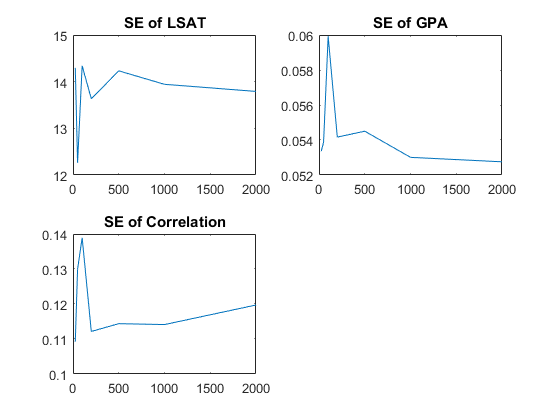
\includegraphics[scale=1]{hw31b.png}\\
\medskip

(c)Plot histogram of bootstrap replicates of corr for the case B=2000.\\
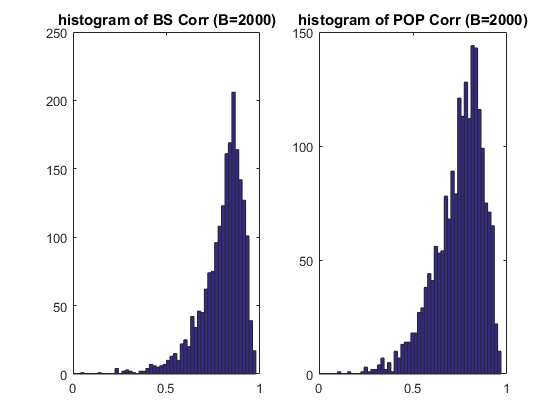
\includegraphics[scale=1]{hw31c.png}\\
The two histogram centered at similar location but the first one(Corr estimates from Bootstrapping) seems to be spikier(smaller standard error). But generally very similar.\\
\bigskip

2. Estimating trimmed mean\\
(a)\\
\begin{tabular}{ c c c c c c c}
 B & 25 & 100 & 200 & 500 & 1000 & 2000\\ 
 SE & 2.2349 & 2.0212 & 1.8934 & 2.0582 & 2.0164 & 2.0564 
\end{tabular}
\medskip

(b)How large should we take B to provide reasonable accuracy.\\
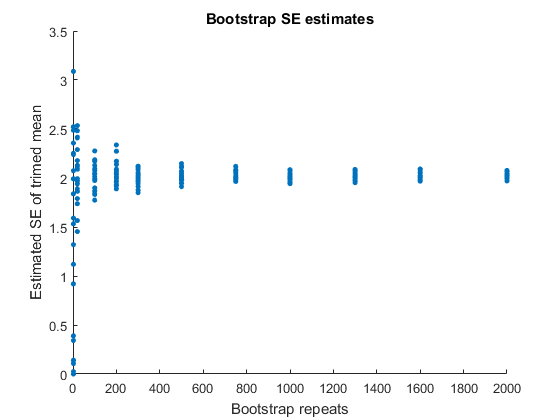
\includegraphics[scale=1]{hw32.png}\\
According to this figure, we can see the estimated of standard error of trimed mean estimator converges quickly when B goes up. And when B is above 1000, it seems good enough.\\ 
\bigskip

3. Estimating the bias of median estimating the mean.\\
I use 1000 repeats for bootstrap median estimate. \\
when n=10, Bias=0.0906\\
when n=20, Bias=0.1063\\
when n=100, Bias=-0.0574\\
The bias is based on the sample we simulated from the normal distribution.\\  

All code please see https://github.com/rikku1983/STAT5376\\
\bigskip

Thanks!


\end{document}